\subsection{UC-0}

\begin{figure}[H]
    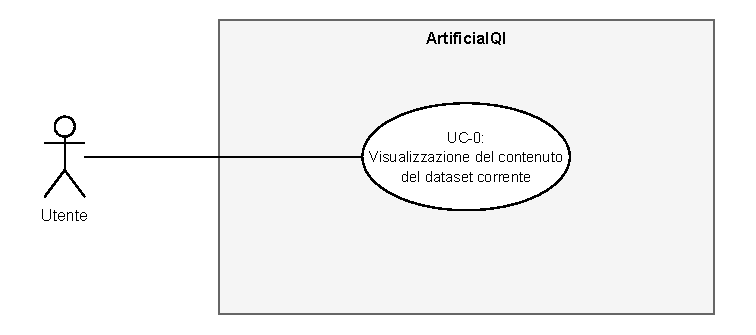
\includegraphics{Sezioni/UseCase/Immagini/UC-0.pdf}
    \caption{Diagramma UC-0.}
\end{figure}

\begin{usecase}{UC-0}{Visualizzazione di un dataset}
    
    \req{\hyperref[item:RU-1]{RU-1}} 

    \pre{
        \item Il sistema è attivo e funzionante
        \item Il dataset esiste
    }

    \post{
        \item Viene visualizzato il dataset
    }
    
    \actor{Utente}

    \subactors{}

    \trigger{L'utente deve visualizzare il dataset}
    
    \inc{}

    \base{}

    \scenario{
        \item L'utente richiede la visualizzazione del dataset
        \item Le coppie del dataset vengono mostrate in una lista
    }

    \subscenario{
        \item[2.1] \textbf{Il dataset è vuoto}
        \begin{itemize}
            \item[a.] Viene indicato all'utente che il dataset è vuoto
        \end{itemize}
    }
\end{usecase}